%\section{Algorithm: choosing when and what to query}
%\label{sec:async}
%
%% Restate our goal
%We now return to task of minimizing the objective in \equationref{objective}.
%For a single input $\bx\oft t$, we must optimize over a set of queries $Q\oft{t}$ to minimize the single-step loss:
%\begin{align*}
%  \ell\oft{t} &= \min_{Q\oft{t}} \ell_{\rmclass}(\by\oft{t}, \byt\oft{t}) + C(Q\oft{t}, \tau\oft{t}) \\
%  Q\oftt{t}{*} &= \argmin_{Q\oft{t}} \ell_{\rmclass}(\by\oft{t}, \byt\oft{t}) + C(Q\oft{t}, \tau\oft{t}),
%\end{align*}
%where $\byt\oft t = \argmin_{\by} \p(\by \given \bx \oft t, \bz\oft t)$ is the MAP estimate given responses $\bz\oft t$ and $\tau\oft t$ is the time taken to execute the queries.
%
%The choice of $Q\oft{t}$ can be reduced to a sequence of queries: $q_1, q_2, \ldots q_m \in \{1, \ldots, n\}$, where $n$ is the size of the output $\by\oft{t}$.
%To keep things tractable, let $Q\oft{t}$ be constructed by picking one query at a time:
%given that we have already made queries $q_1, \ldots, q_{m-1}$, we choose the next query $q_m$ to optimize the loss,
%\begin{align}
%  q_m^* &= \argmin_{q_m \in \{\emptyset, 1, \ldots n\}} \ell_{\rmclass}(\by\oft{t}, \byt\oft{t}) + C((q_1, \ldots, q_m), \tau(q_1, \ldots, q_m)), \label{eqn:one-step-q}
%\end{align}
%where we have extended the domain of $q_m$ to include the symbol $\emptyset$ that denotes {\em not\/} making a query, and returning the current prediction.
%
%We can not yet optimize \equationref{one-step-q} because we do not observe $\by\oft t$ or $\tau\oft t$ ahead of time.
%Instead, we propose to optimize the expected loss under our model, {\em given the responses $\bz$ received when making the decision}.
%For example, if we choose $q_m$ before receiving responses from the previous queries $q_{1:m-1}$ we can optimize the following expression:
%\begin{align}
%  q_m^* &= \argmin_{q_m \in \{\emptyset, 1, \ldots n\}} 
%  \E_{z_1, z_2, \ldots, z_{m}}[\E_{\by \sim \p(\cdot \given \bx\oft t, z_1, \ldots z_m)}[\ell_{\rmclass}(\by, \byt\oft{t})]] + \E_{\tau}[C((q_1, \ldots, q_m), \tau)]. \label{eqn:cumbersome}
%\end{align}
%The expressions to choose $q_m$ after waiting for some responses are cumbersome, but can be easily represented using an expectimin tree.
%
%\begin{figure}
% 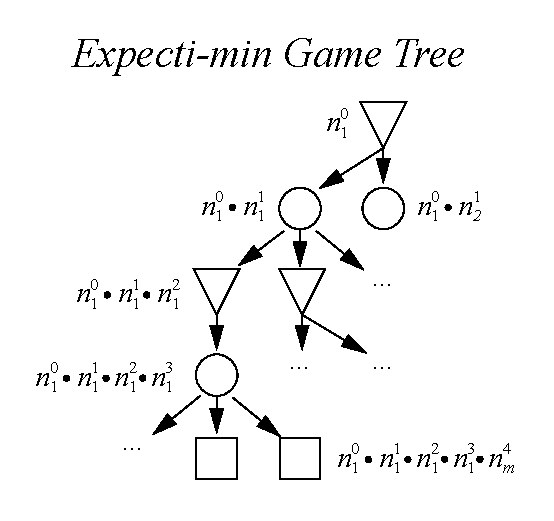
\includegraphics[width=0.49\textwidth,height=0.23\textheight,keepaspectratio]{figures/game-tree.pdf}
%  \hfill
% 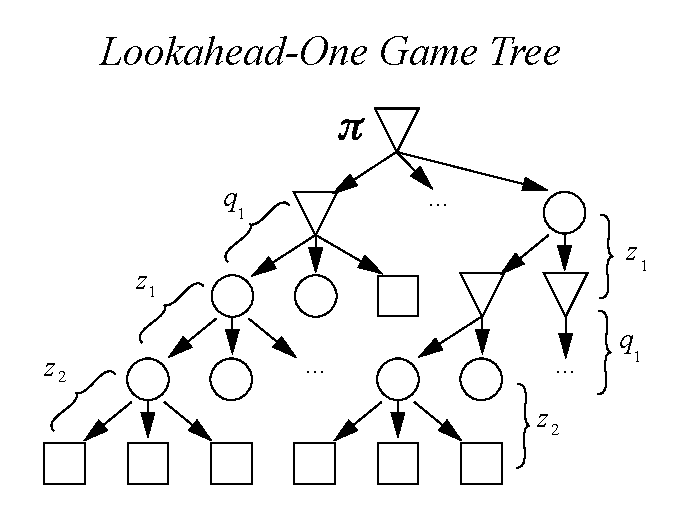
\includegraphics[width=0.49\textwidth,height=0.23\textheight,keepaspectratio]{figures/lookahead-one.pdf}
%  \caption{Monte Carlo tree search}
%\label{fig:mcts}
%\end{figure}
%
%\paragraph{Expectimin trees and optimal policies.}
%Let $\sT(\sN)$ be a expectimin tree with nodes $\sN$ (\figureref{mcts}).
%Each node $n \in \sN$ has a type $n.\sctype$ which is one of $\scmin$ (represented with inverted triangles), $\scexpect$ (represented with circles) or $\scvalue$ (represented with a square) and has children $n.\scchildren \subset \sN$.
%Additionally, nodes of type $\scvalue$ have a value $n.\scvalue$.
%The value of a node can be easily computed recursively: 
%\begin{align*}
%  \scvalue(n) &=
%  \begin{cases}
%    \min_{n'\in n.\scchildren} \scvalue(n') & \textrm{if}~n.\sctype = \scmin \\
%    \E_{n'\sim n.\scchildren}[\scvalue(n')] & \textrm{if}~n.\sctype = \scexpect \\
%    n.\scvalue & \textrm{if}~n.\sctype = \scvalue
%  \end{cases}.
%\end{align*}
%Additionally, an expectimin policy $\pi^*$ at a $\scmin$ node returns the child with the minimum value: $\pi^*(n) = \argmin_{n' \in n.\scchildren} \scvalue(n')$.
%As a concrete example, consider the expectimin tree in \figureref{mcts}. The value of the root node $n_1^0$ is,
%\begin{align*}
%  \scvalue(n_1^0) &= \min_{n_1^0.n_i^1} \E_{n_1^0.n_i^1.n_j^2} \left[\min_{n_1^0.n_i^1.n_j^2.n_k^3} \E_{n_1^0.n_i^1.n_j^2.n_k^3.n_l^4} \left[n_1^0.n_i^1.n_j^2.n_k^3.n_l^4.\scvalue \right] \right].
%\end{align*}
%
%\paragraph{Choosing queries $q_m$ with an expectimax tree.}
%Let us now formalize our decision problem as an expectimin tree, $\sT$.
%The nodes of the tree need to encapsulate as current state, the current time, $t$, the list of queries pending responses $Q = \{(q_1, t_1), \ldots, (q_m, t_m)\}$, where $q_i$ are the queries and $t_i$ is the time at which the query responds (we will compute an expectation over this quantity) and the received responses $Z = \{z_1, \ldots, z_l\}$.
%Without loss of generality, assume that $Q$ is sorted so that $t_1$ is closest in time to $t$.
%Let the root of $\sT$ be the $\min$ node $\scchoose(t, Q, Z)$, 
%with children $\scchoose(t, Q, Z).\turnin$, $\scchoose(t, Q, Z).\wait$ and $\scchoose(t, Q, Z).\query(q)$ for $q \in [n]$.
%$\scchoose(t, Q, Z).\turnin$ is a $\scvalue$ node with value equal to the expected loss of making a prediction in the current state:
%\[
%\scchoose(t, Q, Z).\turnin.\scvalue 
%= \E_{\by \sim \p(\cdot \given \bx, Z)}[\ell_{\rmclass}(\by, \byt)] + C(Q, t).
%\]
%$\scchoose(t, Q, Z).\wait$ is an $\scexpect$ node children $\{\scchoose(t', Q', Z') | t' = t_1, Q' = Q \setminus (q_1, t_1) Z' = Z \union {z_{l+1}} \forall z_{l+1} \in [L]\}$.
%Intuitively, choosing the $\wait$ node waits for the next response by advancing time and updating the query and response states.
%Finally,
%$\scchoose(t, Q, Z).\query(q)$ is an $\scexpect$ node that results in children 
%$\{\scchoose(t, Q', Z) | Q' = Q \union (q, t'), t' = t + \tau_q, \tau_q \sim \Gamma\}$: the $\query$ node places a new query and its expected time of response to $Q$. 
%
%\figureref{mcts} shows a simplified tree ignoring time constructed with a single query in flight; the root node is $\scchoose(\cdot, \{(q_1, t_1)\}, \{\})$. The branch on the left shows the expansion of the game tree along the child that chooses to query immediately, while the branch on the right considers the case where we wait to receive the first response ($z_1$) before querying ($q_2$).
%In the latter scenario, we may choose not to query again if the response we receive provides enough information.

%As described in \sectionref{model}, we would like to select and schedule several requests for labels to maximize our accuracy on predictions while trading off the cost and response time. 
%We view the problem in the Bayesian decision theoretic setting: what is the optimal behavioral policy under our current beliefs?
%The delay in the information we receive from label requests requires us to reason about time and the possible interactions between the responses we will receive.
%In this section, we describe how these interactions can be described using an expectimax tree.
%However, evaluating the optimal policy from the expectimax tree is intractable.
%We propose a Monte Carlo search based algorithm to efficiently approximate the optimal policy.

\paragraph{Efficient Monte Carlo approximation.}

Computing the optimal policy is intractable, especially because of the addition of continuous time.
We propose an approximate algorithm that combines ideas from both TD learning
\citep{sutton1988learning} and Monte Carlo Tree Search (MCTS)
\citep{kocsis2006bandit}, which have been successful in game playing.
Our algorithm
uses the UCT decision rule of MCTS but instead of estimating a separate value for each node,
we use a parametrized value function to share information across nodes:
$V(s) = w \cdot \psi(s)$, where $\psi$ are features of the state $s$ and $w$ are learned weights.
\algorithmref{mcvts} gives the pseudocode of our approach.
On the system's turn, we choose the action that maximizes
the sum of two terms: the first corresponding to the estimated value (exploitation),
and the second depending on the number of visits (exploration).
On the crowd's turn, we sample from distribution given by the simulation dynamics model.

%Briefly, Monte Carlo tree search estimates values of $\scexpect$ nodes by sampling its children.
%The UCT decision heuristic treats each $\scmin$ node as a bandit problem and discovers the child with minimum value.
%However, $\sT$ contains an infinite number of $\scmin$ nodes corresponding to each point in time. 
%Intuitively, we expect that the value of these $\scmin$ nodes are highly correlated and should share information.
%As a separate insight, our model should give us a lot of information about the value of different queries through the marginals which can again help prevent the unnecessary sampling of poor arms.
%We capture these two pieces of information by approximating the value of a state with a linear function, $\scvalue^f(n)$. 
%A typical choice for the features $\sigma(n)$ are the label marginals and time.

%We propose using a variant of the Monte Carlo tree search algorithm\needcite{} \algorithmref{value} that featurizes state.
%Monte Carlo tree search using the UCT algorithm requires each action to be sampled at least once.
%However, each action requires an additional marginal inference step, making sampling expensive.
%We use computed marginals as features to estimate value of each action without ever sampling that action.
%
%In the active learning setting, our model gives us a lot of information about what to query, and we should use it.
%We incorporate the models marginals and time into features and use it to query.
%Instead of storing values in the expectimax nodes, we compute it using a linear value function, $V(s) = \theta^\top \phi(s)$.
%This is similar to approach followed in Dyna-2.
%Algorithm X shows you what to do.

\begin{algorithm}
%  \renewcommand{\algorithmicrequire}{\textbf{Input:}}
%  \renewcommand{\algorithmicensure}{\textbf{Output:}}
\caption{Approximating the value with TD learning and MCTS}
\label{algo:mcvts}
  \begin{algorithmic}[1]
    \Function{monteCarloValue}{state $s$}
    \If{\text{system's turn}}
    \State $s' \gets \argmax_{s'} \left\{V(s') + c \sqrt{\frac{\log N(s)}{N(s')}} \right\}$
      \Comment Choose child using UCT
      \State $v \gets $\Call{monteCarloValue}{$s'$}
      \State $w \gets w + \alpha (v - V(s')) \nabla_w V(s')$
      \Comment Update value function approximation
      \State increment $N(s)$ and $N(s')$
      %\State $n.\scvisits \gets n.\scvisits + 1, n'.\scvisits \gets n'.\scvisits + 1$
      \State \Return $v$
    \ElsIf{crowd's turn}
      \State $s'$ drawn based on (\ref{eqn:dynamics})
      \Comment Sample a child
      \State \Return \Call{monteCarloValue}{$s'$}
    \ElsIf{leaf node}
    \State \Return utility $U$ of $s$ according to (\ref{eqn:utility})
    \EndIf
    \EndFunction{}
    %\Function{$\scvalue^f$}{node $n$}
      %\State \Return $\theta^\top \phi(n)$
      %\Comment Linear function approximation
    %\EndFunction{}
  \end{algorithmic}
\end{algorithm}

%\pldone{Instead of writing down equations,
%cast this as a game tree from the beginning with actions, possible feedback, etc.
%Draw a nice example.
%Then expected utility, expectimax policy, etc. should be conceptually obvious.
%}{Lots of game trees!}

% -- EVERYTHING BELOW THIS IS DEAD TO ME. --
% Let $\ell(\by, \byt)$ be the loss incurred when if $\by$ is labeled $\byt$.
% When presented with an example $\bx$ to label, our system estimates a loss of $\E_{p(\by \given \bx)}[\ell(\by, \byt)]$, where $\byt = \argmin_{\by} \p(\by \given \bx)$.
% If we performed the measurement operator $\sigma$ and received a measurement $\tau$,
% then our expected loss would be $\E_{p(\by \given \bx, \tau)}[\ell(\by, \byt(\tau))]$, where $\byt(\tau) = \argmin_{\by} p(\by \given \bx, \tau)$.
% Intuitively, if we had perfect feedback, observing $\tau$ would provide use more information, reducing our risk.
% However, taking measurements has an associated cost, $C(\sigma)$, a function of time and money that the designer must choose.
% There is also a possibility that the measurement does not return a value (because of a timeout).
% 
% Let the CDF be $F_\sigma(t)$.
% We model the utility of a particular measurement operation, given a time window $t_0$ to be:
% \begin{align*}
% U(\sigma)
% &= F_\sigma(t_0) 
%   \E_{p(\tau \given x, \sigma)} \left[\E_{p(\by \given \bx, \tau)}[\ell(\by, \byt(\tau))] \right]
%   + (1 - F_\sigma(t_0)) 
%     \left[\E_{p(\by \given \bx)}[\ell(\by, \byt)] \right]
%   + C(\sigma).
% \end{align*}
% \pl{too abstract!  I know the measurements paper was a bit abstract...do as I say, not as I did}
% 
% Without loss of generality, assume that the null measurement is free: $C(\sigma_0) = 0$.
% Intuitively, this ensures that we will only ever choose to measure something if the expected reduction in risk is more than the cost of executing the measurement.
% 
% Let the label $\by$ have $n$ components: $\by = (y_1, ..., y_n)$.
% Further, let us assume that the loss function $\ell$ decomposes over labels: $\ell(\by, \byt) = \sum_{i=1}^n \ell(y_i, \yt_i)$. 
% Under this assumption, the expected utility of a single measurement operator $\sigma$ can be efficiently computed with $2L$ inference calls\footnote{The marginal inference query in lines 6 and 7 of \algorithmref{expected-utility} can be shared.} to the model using \algorithmref{expected-utility}.
% 
% The measurement operator to take is simply $\sigma^* = \argmin_{\sigma \in \Sigma} U(\sigma)$.
% 
% \begin{algorithm}
% \renewcommand{\algorithmicrequire}{\textbf{Input:}}
% \renewcommand{\algorithmicensure}{\textbf{Output:}}
%   \caption{Computing expected utility $U(\sigma)$}
%   \label{algo:expected-utility}
%   \begin{algorithmic}[1]
%     \REQUIRE Measurement operator $\sigma$, input $\bx$, models $p_\theta(\by \given \bx)$ and $p_\theta(\by \given \bx, \tau, \sigma)$, $F_\sigma$ and $t_0$.
%     \ENSURE Expected utility $U(\sigma)$
%     \STATE Let $y_\sigma$ be label(s) measured by operator $\sigma$.
%     \STATE Compute $p_\theta(y_\sigma \given \bx)$ using marginal inference.
%     \STATE Set $p_\theta(\tau \given \bx) \gets p_\theta(\tau \given y_\sigma, \bx) p_\theta(y_\sigma \given \bx)$.
%     \STATE Initialize $u \gets (0, \dots, 0)$.
%     \FORALL{$i \in [L]$}
%     \STATE Compute $\byt = \argmin_{\by} p_\theta(\by \given \bx, \tau = i, \sigma)$ using marginal inference.
%     \STATE Compute $p(y_j) = p_\theta(\by_j \given \bx, \tau = i, \sigma)$ for $j \in [n]$ using marginal inference.
%     \STATE Update $u[i] \gets \p(\tau = i \given \bx) \E_{p(y_j)}[\ell(y_j, \yt_j)]$.
%     \ENDFOR
%     \STATE Return the expected utility: $\frac{\sum_{i=1}^L u[i] p_\theta(\tau = i \given x)}{\sum_{i=1}^L p_\theta(\tau = i \given x)}$
%   \end{algorithmic}
% \end{algorithm}
% 
% From a practical perspective, we need to execute multiple queries. We consider this in \sectionref{async}.
% 
% 
% 
% For the system to be real-time, we need to dispatch multiple measurement queries at the same time.
% Let $\sigma_1, \sigma_2, \dots, \sigma_n$ be the set of queries we can dispatch.
% 
% \begin{note}[Baseline: Next best policy]
% \noteb{(arun): We should probably move this to experiments as a baseline or ignore all together.}
% In this scheme we do not reason about the future and choose subsequent measurement operators by going down the ordered list of measurement utilities.
% This approach, while simple, does not allow us to query the same node multiple times, which is often optimal if there is high uncertainty on a single important node.
% \end{note}
% 
% We need to reason about the possible responses that might be returned.
% For the sake of simplicity, we will choose (sequentially) the best set of $n$ measurements to make at the very beginning of our time window, not taking into account responses.
% 
% \algorithmref{expected-utility} can be trivially updated by incorporating previous measurement operators, say $\tau_1, \dots, \tau_{n-1}$.
% Naively, this would require us to enumerate over $L^d$ possible values of $\tau_1, \dots, \tau_n$ in line 5 of \algorithmref{expected-utility}.
% Instead, we propose using a particle filter to estimate utilities (\algorithmref{filtered-utility}).
% 
% \begin{algorithm}
% \renewcommand{\algorithmicrequire}{\textbf{Input:}}
% \renewcommand{\algorithmicensure}{\textbf{Output:}}
% \caption{Computing expected utility $U(\sigma_n \given \sigma_{1:n-1})$ with a particle filter}
%   \label{algo:expected-utility}
%   \begin{algorithmic}[1]
%     \REQUIRE Measurement operators $\sigma_1, \dots, \sigma_n$, input $\bx$, models $p_\theta(\by \given \bx), \dots, p_\theta(\by \given \bx, \tau_{1:n}, \sigma_{1:n})$
%     \ENSURE Expected utility $U(\sigma_n \given \sigma_{1:n-1})$
%     \STATE Let $y_{\sigma_n}$ be label(s) measured by operator $\sigma_n$.
%     \STATE Initialize $u \gets (0, \dots, 0)$.
%     \FORALL{particles $t \in [T]$}
%       \FORALL{$i \in [n-1]$}
%       \STATE Sample $\tau_i\oft{t} \sim \p(\by \given \bx, \tau_{1:i-1}\oft{t}, \sigma_{1:i})$
%       \ENDFOR
%       \STATE Set $\pi(\tau_n) \gets \p(\tau_n \given \bx, \tau_{1:n-1}\oft{t}, \sigma_{1:n})$.
%       \STATE Initialize $u\oft{t} \gets (0, \dots, 0)$.
%       \FORALL{$\tau_n \in [L]$}
%       \STATE Compute $\byt = \argmin_{\by} p_\theta(\by \given \bx, \tau_{1:n}, \sigma_{1:n})$ using MAP inference.
%       \STATE Compute $p(y_j) = p_\theta(\by_j \given \bx, \tau_{1:n}, \sigma_{1:n})$ for $j \in [n]$ using marginal inference.
%       \STATE Update $u\oft{t}[\tau_n] \gets \E_{p(y_j)}[\ell(y_j, \yt_j)]$.
%       \ENDFOR
%       \STATE Update the expected utility: $u \gets u + \frac{1}{T} \frac{\sum_{i=1}^L u[i] \pi(i)}{\sum_{i=1}^L \pi(i)}$.
%     \ENDFOR
%     \STATE Return the expected utility: $u$.
%   \end{algorithmic}
% \end{algorithm}
% 
% For each measurement, we compute the operator maximizing the expected utility $\sigma_n^* = \argmin U(\sigma_n \given \sigma_{1:n-1})$ until we reach a $\sigma_n^* = \sigma_0$.
% \todo{(arun): BAD NOTATION! The subscripts refer to members of $\Sigma$, but also the sequence of measurements.}
% 
% \pl{I guess the particle filter is out of date;
%   in any case, I think we give one algorithm
% that works on the game tree, and say what the computational complexity of the different operations}
% 
% \subsection{Modeling time}
% \label{sec:time}
% 
% When asking for multiple requests, we must decide between sending a request for information right now versus when we receive the measurement.
% In the latter case, we have more information and can make a better informed decision.
% Provided unlimited time, the latter is always optimal, but realistically, we have a finite time window in which to make decisions.
% 
% We model this.
% 
% \paragraph{Preventing overconfidence!}
% Partial monitoring tells us to just sample randomly with some epsilon rate.
% 
% Alekh~\cite{agarwal2013selective} tells us to sample a random dataset occasionally and then see if it's model is better than the actively sampled one. Sounds a bit stupid to me.
% 
